% Figure 3. What goes in a project write-up. Labels: LABELS.md, Figure 3.
% The path map (Fig 4.1) is reused unchanged and is not drawn here.
\def\eeprepfigure{1}
\providecommand{\eepstyledir}{../style}% repo: ../style
\input{\eepstyledir/circuitikz-preamble.tex}
% Colours, fonts, and text styles for the Get hired figures.
% Input after style/circuitikz-preamble.tex (in the repo: ../../style/circuitikz-preamble.tex).
% Define \eepdark before this file for the dark build. Same names as the resume figures,
% plus the rest of the navy palette. Crimson (eepaccent) marks one thing per figure.
\setmainfont{Newsreader}[
  BoldFont={Newsreader Bold},
  ItalicFont={Newsreader Italic},
  BoldItalicFont={Newsreader Bold Italic},
]
\usetikzlibrary{arrows.meta,calc,decorations.pathreplacing}
\ifdefined\eepdark
  \definecolor{eepink}{HTML}{ECEEF2}
  \definecolor{eeptext}{HTML}{D0D4DB}
  \definecolor{eepinktwo}{HTML}{A6AFBF}
  \definecolor{eepmute}{HTML}{8F95A0}
  \definecolor{eepsilver}{HTML}{76808F}
  \definecolor{eeprule}{HTML}{3B4352}
  \definecolor{eepwash}{HTML}{17243A}
  \definecolor{eepsunken}{HTML}{101828}
  \definecolor{eepfill}{HTML}{131C2E}
  \definecolor{eeppaper}{HTML}{0D1524}
  \definecolor{eepaccent}{HTML}{E06A5F}
  \definecolor{eepaccentsoft}{HTML}{2A1A24}
\else
  \definecolor{eepink}{HTML}{16233A}
  \definecolor{eeptext}{HTML}{232A39}
  \definecolor{eepinktwo}{HTML}{424D63}
  \definecolor{eepmute}{HTML}{5E636C}
  \definecolor{eepsilver}{HTML}{838C9A}
  \definecolor{eeprule}{HTML}{C4C8CF}
  \definecolor{eepwash}{HTML}{E7ECF3}
  \definecolor{eepsunken}{HTML}{F3F4F6}
  \definecolor{eepfill}{HTML}{FFFFFF}
  \definecolor{eeppaper}{HTML}{FBFBFC}
  \definecolor{eepaccent}{HTML}{A3201D}
  \definecolor{eepaccentsoft}{HTML}{F8ECEA}
\fi
% Draw in y-down points so coordinates read like a mockup: [x=1pt, y=-1pt].
\tikzset{
  eeptitle/.style={anchor=base west, inner sep=0pt, text=eepink, font=\rmfamily\bfseries\fontsize{26}{31}\selectfont},
  eephead/.style={inner sep=0pt, text=eepink, font=\sffamily\bfseries\fontsize{14.5}{18}\selectfont},
  eepbody/.style={inner sep=0pt, text=eepinktwo, font=\sffamily\fontsize{13}{17}\selectfont},
  eepnote/.style={inner sep=0pt, text=eepmute, font=\sffamily\fontsize{12.5}{16}\selectfont},
  eepsrc/.style={anchor=north west, inner sep=0pt, align=left, text=eepmute, font=\sffamily\fontsize{11}{14.5}\selectfont},
  eepbox/.style={draw=eepink, fill=eepfill, rounded corners=4pt},
  eepfocus/.style={draw=eepaccent, fill=eepfill, rounded corners=4pt, line width=1.8pt},
  eeparrow/.style={-{Stealth[length=8pt,width=6pt]}},
  eepdash/.style={dash pattern=on 4pt off 4pt},
  eeplead/.style={draw=eepsilver, line width=0.9pt},
}
% A dot on a trace, like a schematic junction.
\newcommand{\eepdot}[2][eepink]{\fill[#1] #2 circle (3.6pt);}
% Short labels never hyphenate.
\hyphenpenalty=10000 \exhyphenpenalty=10000
% One space after a full stop, as on the site.
\frenchspacing

% #1 top y, #2 height, #3 label, #4 style, #5 extra drawing (placeholder text lines)
\newcommand{\block}[5]{%
  \draw[#4] (20,#1) rectangle (434,{#1+#2});
  \node[eephead, anchor=north west] at (36,{#1+14}) {#3};
  #5}
\newcommand{\lines}[1]{% two grey placeholder text lines under a label
  \draw[eeprule, line width=3pt] (36,{#1+42}) -- (360,{#1+42}) (36,{#1+54}) -- (290,{#1+54});}
\begin{document}
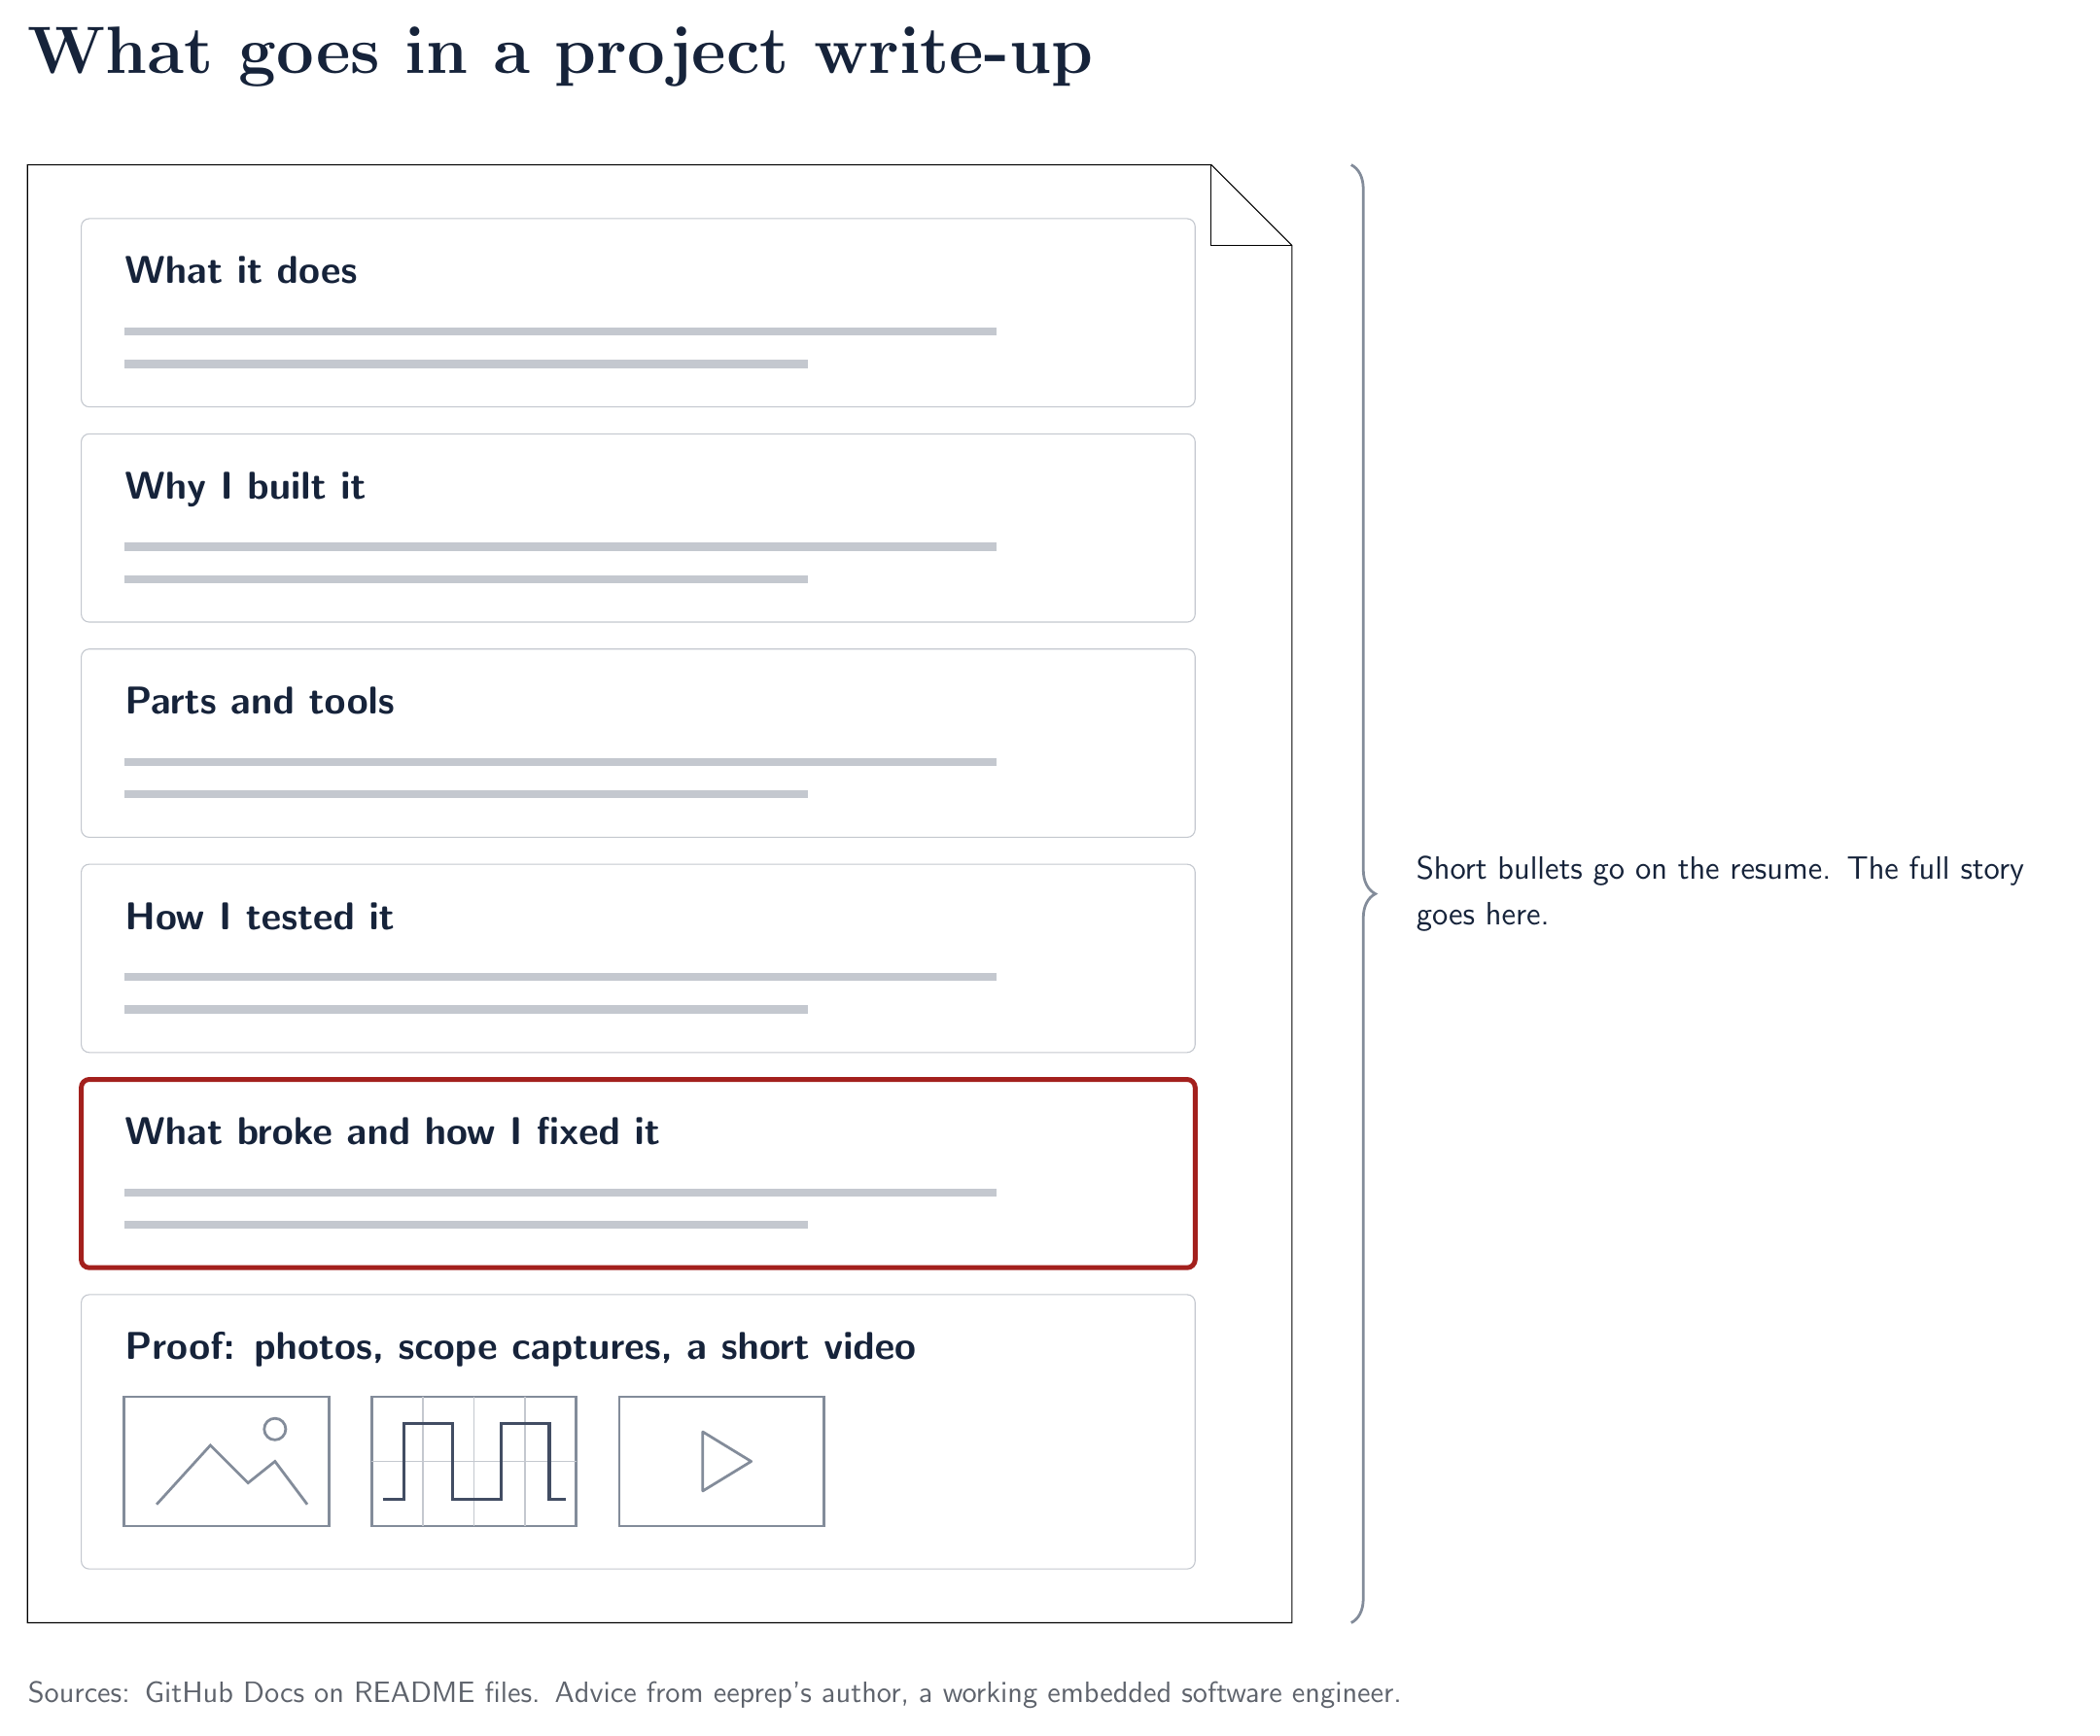
\begin{tikzpicture}[x=1pt,y=-1pt]
  \node[eeptitle] at (0,30) {What goes in a project write-up};
  % One page, like a README, with a folded corner.
  \draw[fill=eepfill] (0,64) -- (440,64) -- (470,94) -- (470,606) -- (0,606) -- cycle;
  \draw (440,64) -- (440,94) -- (470,94);
  \block{84}{70}{What it does}{draw=eeprule, rounded corners=3pt}{\lines{84}}
  \block{164}{70}{Why I built it}{draw=eeprule, rounded corners=3pt}{\lines{164}}
  \block{244}{70}{Parts and tools}{draw=eeprule, rounded corners=3pt}{\lines{244}}
  \block{324}{70}{How I tested it}{draw=eeprule, rounded corners=3pt}{\lines{324}}
  \block{404}{70}{What broke and how I fixed it}{draw=eepaccent, line width=1.8pt, rounded corners=3pt}{\lines{404}}
  \block{484}{102}{Proof: photos, scope captures, a short video}{draw=eeprule, rounded corners=3pt}{%
    % Three thumbnails: a photo, a scope capture, a video.
    \draw[eepsilver, line width=1pt] (36,522) rectangle (112,570);
    \draw[eepsilver, line width=1pt] (48,562) -- (68,540) -- (82,554) -- (92,546) -- (104,562);
    \draw[eepsilver, line width=1pt] (92,534) circle (4pt);
    \draw[eepsilver, line width=1pt] (128,522) rectangle (204,570);
    \draw[eeprule, line width=0.6pt] (147,522) -- (147,570) (166,522) -- (166,570) (185,522) -- (185,570) (128,546) -- (204,546);
    \draw[eepinktwo, line width=1.2pt] (132,560) -- (140,560) -- (140,532) -- (158,532) -- (158,560) -- (176,560) -- (176,532) -- (194,532) -- (194,560) -- (200,560);
    \draw[eepsilver, line width=1pt] (220,522) rectangle (296,570);
    \draw[eepsilver, line width=1pt, line join=round] (251,535) -- (251,557) -- (269,546) -- cycle;}
  % Side note, pointing at the whole page.
  \draw[eepsilver, line width=1pt, decorate, decoration={brace, amplitude=9pt}] (492,64) -- (492,606);
  \node[eepbody, anchor=west, text width=240pt, align=left, text=eepink] at (516,335) {Short bullets go on the resume. The full story goes here.};
  \node[eepsrc, text width=760pt] at (0,628) {Sources: GitHub Docs on README files. Advice from eeprep's author, a working embedded software engineer.};
\end{tikzpicture}
\end{document}
